\SourcePage{331}{334}
\section{Mendeleev's periodic system of the elements}

To explain the periodic variation of properties discovered by D.~I.~Mendeleev (1869) among elements arranged in order of increasing atomic number, one must examine the special features of the successive filling of atomic electron shells (N.~Bohr, 1922).

\SourcePage{332}{335}
In passing from one atom to the next, the charge increases by one unit and one electron is added to the shell. At first sight, one might expect the binding energies of successively added electrons to change monotonically as the atomic number rises. In fact, this is not so.

The normal state of the hydrogen atom contains only one electron, in the $1s$ state. In the atom of the next element, helium, another electron is added in the same $1s$ state. The binding energy of each $1s$ electron in helium is, however, much greater than the binding energy of the electron in hydrogen. This follows naturally from the difference between the field experienced by an electron in H and the field encountered by an electron added to a He$^+$ ion: far from the nucleus the two fields are approximately the same, but near the nucleus the field of the He$^+$ ion, whose charge is $Z=2$, is stronger than that of the hydrogen nucleus with $Z=1$.

In lithium ($Z=3$), the third electron enters the $2s$ state, since no more than two electrons can occupy the $1s$ states at the same time. For a specified $Z$, the $2s$ level lies above the $1s$ level; both fall as the nuclear charge increases. In going from $Z=2$ to $Z=3$, however, the first effect greatly outweighs the second, so that the binding energy of the third electron in Li is much smaller than that of the electrons in helium. Next, from Be ($Z=4$) through Ne ($Z=10$), one further $2s$ electron and then six $2p$ electrons are added in succession. Because the nuclear charge is increasing, the binding energies of the electrons added along this sequence rise on the whole. The next electron, added on passing to Na ($Z=11$), occupies the $3s$ state; here the effect of entering a higher shell outweighs that of the increased nuclear charge, and the binding energy once more drops sharply.

This pattern of shell filling is characteristic of the entire sequence of elements. All electron states can be divided into groups that fill successively. While each group is being filled along the sequence, the binding energy generally rises, but it falls sharply when filling of the next group begins.

Figure~24 plots the ionization potentials of the elements known from spectroscopic data; they determine the binding energies of the electrons added in passing from each element to the next.

\SourcePage{333}{336}
\begin{figure}[ht]
\centering
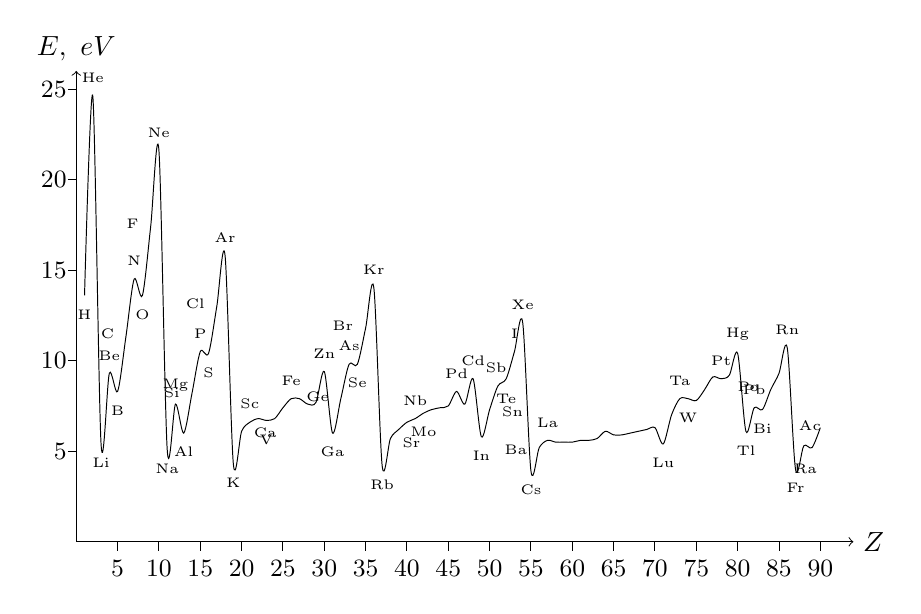
\begin{tikzpicture}[x=.105cm,y=.23cm,line width=.35pt]
 \draw[->] (0,0)--(94,0) node[right] {$Z$};
 \draw[->] (0,0)--(0,26) node[above] {$E,\ \text{eV}$};
 \foreach \y in {5,10,15,20,25} \draw (-1,\y)--(0,\y) node[left] {\small\y};
 \foreach \x in {5,10,...,90} \draw (\x,0)--(\x,-.5) node[below] {\small\x};
 \draw plot[smooth] coordinates {(1,13.6)(2,24.6)(3,5.4)(4,9.3)(5,8.3)(6,11.3)(7,14.5)(8,13.6)(9,17.4)(10,21.6)(11,5.1)(12,7.6)(13,6.0)(14,8.2)(15,10.5)(16,10.4)(17,13.0)(18,15.8)(19,4.3)(20,6.1)(21,6.6)(22,6.8)(23,6.7)(24,6.8)(25,7.4)(26,7.9)(27,7.9)(28,7.6)(29,7.7)(30,9.4)(31,6.0)(32,7.9)(33,9.8)(34,9.8)(35,11.8)(36,14.0)(37,4.2)(38,5.7)(39,6.2)(40,6.6)(41,6.8)(42,7.1)(43,7.3)(44,7.4)(45,7.5)(46,8.3)(47,7.6)(48,9.0)(49,5.8)(50,7.3)(51,8.6)(52,9.0)(53,10.5)(54,12.1)(55,3.9)(56,5.2)(57,5.6)(58,5.5)(59,5.5)(60,5.5)(61,5.6)(62,5.6)(63,5.7)(64,6.1)(65,5.9)(66,5.9)(67,6.0)(68,6.1)(69,6.2)(70,6.3)(71,5.4)(72,7.0)(73,7.9)(74,7.9)(75,7.8)(76,8.4)(77,9.1)(78,9.0)(79,9.2)(80,10.4)(81,6.1)(82,7.4)(83,7.3)(84,8.4)(85,9.3)(86,10.7)(87,4.0)(88,5.3)(89,5.2)(90,6.3)};
 \foreach \x/\y/\t in {2/24.6/He,4/9.3/Be,7/14.5/N,10/21.6/Ne,12/7.6/Mg,15/10.5/P,18/15.8/Ar,21/6.6/Sc,26/7.9/Fe,30/9.4/Zn,33/9.8/As,36/14/Kr,41/6.8/Nb,46/8.3/Pd,48/9/Cd,50.8/8.6/Sb,53/10.5/I,54/12.1/Xe,57/5.6/La,73/7.9/Ta,78/9/Pt,80/10.4/Hg,82/7.4/Pb,86/10.7/Rn,88.75/5.4/Ac} \node[font=\tiny,anchor=south] at (\x,\y+.2) {\t};
 \foreach \x/\y/\t in {1/13.6/H,3/5.4/Li,5/8.3/B,8/13.6/O,11/5.1/Na,13/6.0/Al,16/10.4/S,19/4.3/K,23/6.7/V,31/6.0/Ga,34/9.8/Se,37/4.2/Rb,42/7.1/Mo,49/5.8/In,52/8.95/Te,55/3.9/Cs,71/5.4/Lu,74/7.9/W,81/6.1/Tl,83/7.3/Bi,87/4/Fr,88.2/5.05/Ra} \node[font=\tiny,anchor=north] at (\x,\y-.25) {\t};
 \foreach \x/\y/\t in {5.75/11.5/C,8.7/17.55/F,13.7/8.2/Si,16.7/13.15/Cl,31.75/8.0/Ge,34.65/11.9/Br,55.7/5.1/Ba,83.75/8.55/Po} \node[font=\tiny,anchor=east] at (\x,\y) {\t};
 \foreach \x/\y/\t in {20.3/6.0/Ca,38.3/5.45/Sr,50.35/7.15/Sn} \node[font=\tiny,anchor=west] at (\x,\y) {\t};
\end{tikzpicture}
\caption{}
\label{fig:ionization-potentials}
\end{figure}

\SourcePage{334}{337}
The states are divided among the successively filled groups as follows:
\begin{equation}
\begin{array}{r@{\ }l}
1s&2\text{ electrons},\\
2s,\,2p&8\text{ electrons},\\
3s,\,3p&8\text{ electrons},\\
4s,\,3d,\,4p&18\text{ electrons},\\
5s,\,4d,\,5p&18\text{ electrons},\\
6s,\,4f,\,5d,\,6p&32\text{ electrons},\\
7s,\,6d,\,5f&\ldots
\end{array}
\tag{73.1}
\end{equation}
The first group is filled in H and He. Filling the second and third gives the first two short periods of the periodic system, each containing 8 elements. They are followed by two long periods of 18 elements each and by a long period that includes the rare-earth elements and contains 32 elements in all. The last group of states is not completely filled in the naturally occurring elements (or in the artificially produced transuranium elements).

To understand how the properties change while each group of states is being filled, the following feature of the $d$ and $f$ states, which distinguishes them from the $s$ and $p$ states, is important. For an electron in a heavy atom, the effective-potential-energy curves of the spherically symmetric field (the sum of the electrostatic and centrifugal fields) descend rapidly and almost vertically near the origin, have a deep minimum, and then begin to rise, approaching zero asymptotically. On their rising branches, the curves for the $s$ and $p$ states lie very close together. Thus an electron in either kind of state is located at approximately the same distance from the nucleus. The curves for the $d$ states, and especially the $f$ states, lie considerably farther to the left; the classically allowed region bounded by them ends much nearer the nucleus than it does for $s$ and $p$ states at the same total electron energy. In other words, an electron in a $d$ or $f$ state is found mainly much closer to the nucleus than one in an $s$ or $p$ state.

A number of atomic properties (including the chemical properties of the elements; see \S~81) depend chiefly on the outer regions of the electron shells. The feature of the $d$ and $f$ states just described is therefore highly significant. For example, when the $4f$ states are being filled (in the rare-earth elements; see below), the added electrons lie much closer to the nucleus than the electrons in states filled earlier. Consequently,

\SourcePage{335}{338}
these electrons have almost no effect on chemical properties, and all the rare-earth elements are consequently very similar chemically.


Elements whose $d$ and $f$ shells are filled (or which have no such shells at all) are called \emph{main-group elements}; those in which these states are currently being filled are called \emph{transition-group elements}. It is convenient to discuss the elements of these groups separately.

We begin with the main-group elements. Hydrogen and helium have the normal states
\[
 {}_1\mathrm H\ 1s\,{}^2S_{1/2};\qquad {}_2\mathrm{He}\ 1s^2\,{}^1S_0
\]
(the subscript to the left of a chemical symbol always denotes the atomic number). The electron configurations of the remaining main-group elements are given in Table~3.

\begin{table}[ht]
\centering\small
\caption{Electron configurations of the main-group elements}
\begin{tabular}{c|cccccccc|l}
&$s$&$s^2$&$s^2p$&$s^2p^2$&$s^2p^3$&$s^2p^4$&$s^2p^5$&$s^2p^6$&\\\hline
$n=2$&$_3$Li&$_4$Be&$_5$B&$_6$C&$_7$N&$_8$O&$_9$F&$_{10}$Ne&$1s^2$\\
3&$_{11}$Na&$_{12}$Mg&$_{13}$Al&$_{14}$Si&$_{15}$P&$_{16}$S&$_{17}$Cl&$_{18}$Ar&$2s^22p^6$\\
4&$_{19}$K&$_{20}$Ca&&&&&&&$3s^23p^6$\\
4&$_{29}$Cu&$_{30}$Zn&$_{31}$Ga&$_{32}$Ge&$_{33}$As&$_{34}$Se&$_{35}$Br&$_{36}$Kr&$3d^{10}$\\
5&$_{37}$Rb&$_{38}$Sr&&&&&&&$4s^24p^6$\\
5&$_{47}$Ag&$_{48}$Cd&$_{49}$In&$_{50}$Sn&$_{51}$Sb&$_{52}$Te&$_{53}$I&$_{54}$Xe&$4d^{10}$\\
6&$_{55}$Cs&$_{56}$Ba&&&&&&&$5s^25p^6$\\
6&$_{79}$Au&$_{80}$Hg&$_{81}$Tl&$_{82}$Pb&$_{83}$Bi&$_{84}$Po&$_{85}$At&$_{86}$Rn&$4f^{14}5d^{10}$\\
7&$_{87}$Fr&$_{88}$Ra&&&&&&&$6s^26p^6$\\\hline
&$^2S_{1/2}$&$^1S_0$&$^2P_{1/2}$&$^3P_0$&$^4S_{3/2}$&$^3P_2$&$^2P_{3/2}$&$^1S_0$&
\end{tabular}
\end{table}

In each atom, the shells listed in the rightmost column on the same row, and those on every preceding row, are completely filled. The electron configuration in the shells currently being filled is shown at the top; the principal quantum number of the electrons in these states is the number in the leftmost column of the same row. The normal states of the atom as a whole are shown at the bottom. Thus Al has the electron configuration $1s^22s^22p^63s^23p\,{}^2P_{1/2}$.

The values of $L$ and $S$ in the normal state of an atom can be found (when its electron configuration is known) from

\SourcePage{336}{339}
Hund's rule (\S~67), while $J$ is determined by the rule given in \S~72.

The noble-gas atoms (He, Ne, Ar, Kr, Xe, Rn) occupy a special place in the table: in each of them, the filling of one of the groups of states listed in (73.1) is completed. Their electron configurations are exceptionally stable (their ionization potentials are the largest in the corresponding series). The chemical inertness of these elements is also connected with this stability.


We see that the various states fill in a very regular manner along the sequence of main-group elements: for each principal quantum number $n$, the $s$ states are filled first and the $p$ states next. The electron configurations of ions of these elements are equally regular (as long as ionization does not affect electrons in $d$ and $f$ shells): each ion has the configuration of the preceding atom. Thus Mg$^+$ has the configuration of Na, and Mg$^{++}$ that of Ne.

We now turn to the transition-group elements. The $3d$, $4d$, and $5d$ shells fill in groups of elements known respectively as the \emph{iron}, \emph{palladium}, and \emph{platinum groups}.

Table~4 gives the electron configurations and atomic terms of these groups as established by experimental spectroscopic data. The table shows that the filling of the $d$ shells is much less regular than that of the $s$ and $p$ shells in main-group atoms. Its characteristic feature is a ``competition'' between $s$ and $d$ states. Instead of the regular succession of configurations of the type $d^ps^2$ with increasing $p$, configurations of the form $d^{p+1}s$ or $d^{p+2}$ are often more favourable. In the iron group, for example, Cr has the configuration $3d^54s$ rather than $3d^44s^2$; Ni, with eight $d$ electrons, is followed directly by Cu with a completely filled $d$ shell (and for that reason assigned above to the main groups). The terms of the ions show the same lack of regularity: their electron configurations usually do not coincide with those of the preceding atoms. For example, V$^+$ has the configuration $3d^4$ (not $3d^24s^2$, as in Ti), and Fe$^+$ has $3d^64s$ (rather than the $3d^54s^2$ configuration of Mn). Notice that all ions occurring naturally in crystals and solutions contain only $d$ electrons (and no $s$ or $p$ electrons) in their unfilled shells. Thus iron occurs in crystals or solutions only as Fe$^{++}$ and Fe$^{+++}$ ions, whose configurations are $3d^6$ and $3d^5$, respectively.

\SourcePage{337}{340}
\begin{table}[ht]
\centering\scriptsize
\caption{Electron configurations of atoms in the iron, palladium, and platinum groups}
\begin{tabular}{c|cccccccc}
\multicolumn{9}{c}{Iron group}\\
&$_{21}$Sc&$_{22}$Ti&$_{23}$V&$_{24}$Cr&$_{25}$Mn&$_{26}$Fe&$_{27}$Co&$_{28}$Ni\\
&$3d4s^2$&$3d^24s^2$&$3d^34s^2$&$3d^54s$&$3d^54s^2$&$3d^64s^2$&$3d^74s^2$&$3d^84s^2$\\
&$^2D_{3/2}$&$^3F_2$&$^4F_{3/2}$&$^7S_3$&$^6S_{5/2}$&$^5D_4$&$^4F_{9/2}$&$^3F_4$\\\hline
\multicolumn{9}{c}{Palladium group}\\
&$_{39}$Y&$_{40}$Zr&$_{41}$Nb&$_{42}$Mo&$_{43}$Tc&$_{44}$Ru&$_{45}$Rh&$_{46}$Pd\\
&$4d5s^2$&$4d^25s^2$&$4d^45s$&$4d^55s$&$4d^55s^2$&$4d^75s$&$4d^85s$&$4d^{10}$\\
&$^2D_{3/2}$&$^3F_2$&$^6D_{1/2}$&$^7S_3$&$^6S_{5/2}$&$^5F_5$&$^4F_{9/2}$&$^1S_0$\\\hline
\multicolumn{9}{c}{Platinum group}\\
&$_{57}$La&&&&&&&\\
&$5d6s^2$&&&&&&&\\
&$^2D_{3/2}$&&&&&&&\\
&$_{71}$Lu&$_{72}$Hf&$_{73}$Ta&$_{74}$W&$_{75}$Re&$_{76}$Os&$_{77}$Ir&$_{78}$Pt\\
&$5d6s^2$&$5d^26s^2$&$5d^36s^2$&$5d^46s^2$&$5d^56s^2$&$5d^66s^2$&$5d^76s^2$&$5d^96s$\\
&$^2D_{3/2}$&$^3F_2$&$^4F_{3/2}$&$^5D_0$&$^6S_{5/2}$&$^5D_4$&$^4F_{9/2}$&$^3D_3$
\end{tabular}
\end{table}

The situation is similar when the $4f$ shell is filled, as happens in the sequence of elements called the \emph{rare earths} (Table~5)\footnote{Chemistry texts commonly include Lu among the rare-earth elements as well. This is incorrect, however, since its $4f$ shell is already full; Lu should be assigned to the platinum group, as has been done in Table~4.}. Filling the $4f$ shell is also not entirely regular, being characterized by competition among the $4f$, $5d$, and $6s$ states.

The last group of transition elements begins with actinium. In it the $6d$ and $5f$ shells are filled, in a manner analogous to the filling in the rare-earth sequence (Table~6).

\SourcePage{338}{341}
\begin{table}[ht]
\centering\scriptsize
\caption{Electron configurations of rare-earth atoms}
\begin{tabular}{ccccccc}
$_{58}$Ce&$_{59}$Pr&$_{60}$Nd&$_{61}$Pm&$_{62}$Sm&$_{63}$Eu\\
$4f5d6s^2$&$4f^36s^2$&$4f^46s^2$&$4f^56s^2$&$4f^66s^2$&$4f^76s^2$\\
$^1G_4$&$^4I_{9/2}$&$^5I_4$&$^6H_{5/2}$&$^7F_0$&$^8S_{7/2}$\\\hline
$_{64}$Gd&$_{65}$Tb&$_{66}$Dy&$_{67}$Ho&$_{68}$Er&$_{69}$Tm&$_{70}$Yb\\
$4f^75d6s^2$&$4f^96s^2$&$4f^{10}6s^2$&$4f^{11}6s^2$&$4f^{12}6s^2$&$4f^{13}6s^2$&$4f^{14}6s^2$\\
$^9D_2$&$^6H_{15/2}$&$^5I_8$&$^4I_{15/2}$&$^3H_6$&$^2F_{7/2}$&$^1S_0$
\end{tabular}
\end{table}

\begin{table}[ht]
\centering\scriptsize
\caption{Electron configurations of atoms in the actinide group}
\begin{tabular}{cccccccc}
$_{89}$Ac&$_{90}$Th&$_{91}$Pa&$_{92}$U&$_{93}$Np&$_{94}$Pu&$_{95}$Am&$_{96}$Cm\\
$6d7s^2$&$6d^27s^2$&$5f^26d7s^2$&$5f^36d7s^2$&$5f^46d7s^2$&$5f^67s^2$&$5f^77s^2$&$5f^76d7s^2$\\
$^2D_{3/2}$&$^3F_2$&$^4K_{11/2}$&$^5L_6$&$^6L_{11/2}$&$^7F_0$&$^8S_{7/2}$&$^9D_2$
\end{tabular}
\end{table}

We shall end this section by considering one noteworthy application of the Thomas--Fermi method. We have seen that the first $p$-shell electrons occur in the fifth element (B), that $d$-electrons appear at $Z=21$ (Sc), and that $f$-electrons appear at $Z=58$ (Ce). The Thomas--Fermi method predicts these values of $Z$ in the following way.

In a many-electron atom, an electron of orbital angular momentum $l$ moves with an ``effective potential energy'' equal to\footnote{Atomic units are used, as in \S~70.}

\[
 U_l(r)=-\varphi(r)+\frac{(l+1/2)^2}{2r^2}.
\]
The first term is the potential energy in the electric field described by the Thomas--Fermi potential $\varphi(r)$. The second is the centrifugal energy, in which we write $(l+1/2)^2$ in place of

\SourcePage{339}{342}
$l(l+1)$ because the motion is semiclassical. Since the total energy of an electron in an atom is negative, it is clear that if, for specified $Z$ and $l$, $U_l(r)>0$ for every $r$, the atom cannot contain any electrons at all with the value of $l$ under consideration. If a particular $l$ is fixed and $Z$ is varied, then for sufficiently small $Z$ one indeed finds $U_l(r)>0$ everywhere. As $Z$ is increased, a point is reached at which the curve $U_l=U_l(r)$ touches the abscissa axis; at larger $Z$ there is a region in which $U_l(r)<0$. Thus electrons with a given $l$ first appear in the atom when the curve $U_l(r)$ is tangent to the abscissa axis, that is, when
\[
 U_l(r)=-\varphi(r)+\frac{(l+1/2)^2}{2r^2}=0,
 \qquad U'_l(r)=-\varphi'(r)-\frac{(l+1/2)^2}{r^3}=0.
\]
Substitution of expression (70.6) for the potential gives
\begin{equation}
\begin{split}
 Z^{2/3}\frac{\chi(x)}x&=\left(\frac2{3\pi}\right)^{2/3}\frac{(l+1/2)^2}{2x^2},\\
 Z^{2/3}\frac{x\chi'(x)-\chi(x)}{x^2}&=-2\left(\frac2{3\pi}\right)^{2/3}\frac{(l+1/2)^2}{2x^3}.
\end{split}
\tag{73.2}
\end{equation}
Dividing the second of these equations term by term by the first, we obtain the equation for $x$
\[
 \frac{\chi'(x)}{\chi(x)}=-\frac1x,
\]
after which $Z$ is calculated from the first equation in (73.2). Numerical calculation gives
\[
 Z=0{,}155(2l+1)^3.
\]
This formula determines the values of $Z$ at which electrons with a specified $l$ first appear in the atom (with an error of about 10\%). The exact integer values are obtained if the coefficient 0.155 is replaced by 0.17:
\begin{equation}
 Z=0{,}17(2l+1)^3.
 \tag{73.3}
\end{equation}
For $l=1,2,3$, rounding this formula's results to the nearest integers gives precisely the correct values 5, 21, and 58. For $l=4$, formula (73.3) gives $Z=124$; thus $g$ electrons should first appear only in element 124.
